\thispagestyle{plain}
\section{Resolución de ecuaciones cuadráticas}

\boxabstract{Aprendizajes esperados:}{Resuelve problemas mediante la formulación y la solución algebraica de ecuaciones cuadráticas.}
\subsection{Procedimientos para la resolución de ecuaciones cuadráticas}

\begin{boxK}
    \begin{center}\textbf{Inicio}\end{center}
    \begin{enumerate}
        \item Observa la figura \ref{fig:camino} y responde lo que se pide.
              Un jardín rectangular mide 50 m por 40 m. Se quiere construir un camino de ancho
              constante alrededor del jardín como se muestra en la figura. ¿Qué tan ancho deberá
              ser el camino si debe cubrir un área de 784 m$^2$ ?
              \begin{enumerate}
                  \item Escribe una ecuación que permita obtener el área del camino.
                  \item ¿Cuánto mide el ancho del camino? ¿Cuánta área verde quedará?
                  \item Realiza la gráfica que describe la expresión algebraica obtenida.
                  \item ¿Qué información es relevante para responder y cuál no?
                  \item Describe el procedimiento que realizaste para saber las respuestas.
              \end{enumerate}
        \item Reúnanse en equipo. Reflexionen sobre los procedimientos de solución
              de una ecuación cuadrática. Argumenten. Corrijan si es necesario.
              \begin{figure}[H]
                  \centering
                  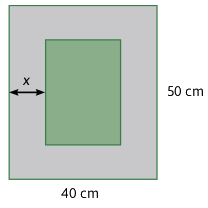
\includegraphics[width=0.4\textwidth]{camino.png}
                  \captionof{figure}{Modelo geométrico de la situación.}
                  \label{fig:camino}
              \end{figure}
    \end{enumerate}
\end{boxK}

\newpage

\subsubsection{Producto de factores lineales}
Responde a los siguientes incisos.
\begin{enumerate}
    \item Considera las ecuaciones $x(x - 9) = 0$ y $x^2 - 9x = 0$.
          \begin{enumerate}
              \item Considera la ecuación $(x)(x) - (9)(x) = 0$ y compárala con $x(x - 9) = 0$. ¿Qué observas? ¿Son equivalentes? Explica.
              \item Efectúa los productos en $(x)(x) - (9)(x) = 0$. ¿Qué expresión obtienes?
              \item ¿Las ecuaciones $x(x - 9) = 0$ y $x^2 - 9x = 0$ son equivalentes? ¿Por qué?
          \end{enumerate}
    \item Considera las ecuaciones $(x + 1)(x - 1) = 0$ y $x^2 - 1 = 0$.
          \begin{enumerate}
              \item Considera la ecuación $(x + 1)(x) + (x + 1)(-1) = 0$ y compárala con
                    $(x + 1)(x - 1) = 0$. ¿Qué observas? ¿Son equivalentes? Explica.
              \item Efectúa los productos en $(x + 1)(x) + (x + 1)(-1) = 0$. ¿Qué expresión obtienes?
              \item ¿Las ecuaciones $(x + 1)(x - 1) = 0$ y $x^2 - 1 = 0$ son equivalentes? ¿Por qué?
          \end{enumerate}

          ¿Cuál es el resultado de efectuar siguientes productos?:
          \[x(x + a)=\]
          \[x(x - a)=\]
          \[(x + a)(x + b)=\]
          \[(x + a)(x - b)=\]
          Supongan que $a$ y $b$ son enteros, fracciones o decimales. Observen con cuidado el manejo de
          los signos al multiplicar.

          \begin{boxH}
              Un \textbf{producto de factores lineales} tiene la forma general de
              \[(ax + b)(cx + d) = acx^2 + adx + bcx + bd = acx^2 + (ad + bc)x + bd\]
          \end{boxH}

          \subsubsection{La factorización para resolver ecuaciones cuadráticas}

          Desarrollaremos la relación que existe entre una ecuación cuadrática escrita como
          producto de expresiones lineales y las soluciones de la ecuación.

    \item Considera las ecuaciones $3x + 2 = 0$ y $x - 4 = 0$.
          \begin{enumerate}
              \item ¿Cuáles son las soluciones de $3x + 2 = 0$ y de $x - 4 = 0$?
              \item Ahora considera la ecuación $(3x + 2)(x - 4) = 0$. ¿Cómo puedes encontrar su solución? ¿Cuál es?
              \item ¿Hay alguna relación entre las soluciones de $3x + 2 = 0$ y $x - 4 = 0$ y las de $(3x + 2)(x - 4) = 0$? Explica.
              \item Efectúa el producto en la ecuación $(3x + 2)(x - 4) = 0$. ¿Qué ecuación obtienes?
              \item ¿Cuáles son las soluciones de la ecuación que obtuviste? ¿Por qué?
          \end{enumerate}

          \newpage

    \item Analiza la ecuación $(x - 1.2) (x + 3.3) = 0$.
          \begin{enumerate}
              \item Efectúen el producto. ¿Qué ecuación obtienen?
              \item ¿Cuáles son las raíces de la ecuación que obtuvieron?
              \item Compara tus respuestas y procedimientos. Si hay diferencias, argumenta. Corrijan si es necesario. Comenten: ¿cómo se relacio-
                    nan las soluciones de una ecuación en la que hay un producto de expresiones li-
                    neales y las de su equivalente ecuación cuadrática?
          \end{enumerate}

          \begin{boxH}
              \textbf{Factorizar} una ecuación cuadrática significa escribirla como el producto de dos
              términos algebraicos lineales. La nueva ecuación es equivalente a la primera y las
              soluciones se obtienen de resolver dos ecuaciones lineales.
              \begin{align*}
                  x^2 + 7x - 18  & = 0 \Rightarrow \\
                  (x + 9)(x - 2) & = 0
              \end{align*}
              y las soluciones a ambas ecuaciones son $x = - 9$ y $x = 2$.
          \end{boxH}

    \item Completa la tabla \ref{tab:table2.6}.

          \begin{figure}[H]
              \centering
              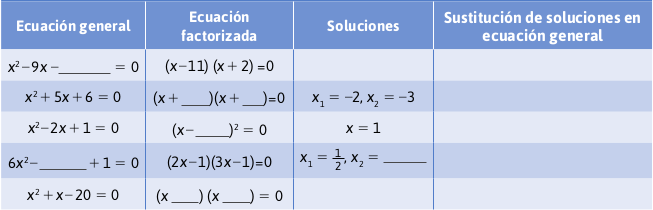
\includegraphics[width=0.9\textwidth]{table2.6.png}
              \captionof{table}{}
              \label{tab:table2.6}
          \end{figure}

          \subsubsection{Técnicas de factorización de ecuaciones cuadráticas}
          Desarrollaremos técnicas sencillas para factorizar ecuaciones cuadráticas.

    \item Desarrollen la ecuación $(x + 8)(x - 3) = 0$. Exprésenla como $ax^2 + bx + c = 0$.
          \begin{enumerate}
              \item ¿Cuál es el valor del coeficiente de $x^2$ ?
              \item ¿Cómo pueden obtener el coeficiente de $x$ con las raíces de $(x + 8)(x - 3) = 0$?
              \item ¿Cómo pueden obtener el término independiente con las raíces de $(x + 8)(x - 3) = 0$?
          \end{enumerate}

    \item Desarrolla la ecuación $(x + r)(x + s) = 0$. Exprésala en la forma $x^2 + bx + c = 0$.
          Consideren que $r$ y $s$ son números enteros, fraccionarios o decimales.
          \begin{enumerate}
              \item ¿Cuál es el valor del coeficiente de $x^2$ ?
              \item ¿Cómo pueden obtener el coeficiente de $x$ con las raíces de $(x + r)(x + s) = 0$?
              \item ¿Cómo pueden obtener el término independiente con las raíces de $(x + r)(x + s) = 0$?
          \end{enumerate}
    \item  Consideren la ecuación $x^2 + 9x + 18 = 0$.
          \begin{enumerate}
              \item ¿Cuáles son los coeficientes de $x^2$ y $x$? ¿Y el término independiente?
              \item Encuentren dos números tales que la suma de ellos sea igual al coeficiente de $x$ y el producto sea igual al término independiente.
              \item Con los números que determinaron, ¿pueden escribir la ecuación $x^2 + 9x + 18 = 0$ como un producto de dos factores lineales? ¿Cómo?
              \item ¿Cómo comprueban que la ecuación $x + 9x + 18 = 0$ y la que escribieron son equivalentes? Háganlo.
          \end{enumerate}

          ¿Cómo factorizan una ecuación cuadrática? ¿Cómo pueden validar su factorización? ¿Cómo pueden
          factorizar ecuaciones del tipo $ax^2 + c = 0$ y $ax^2 + bx = 0$? Propongan varios ejemplos
          y factorícenlos en el pizarrón. Despejen cualquier duda de sus compañeros. Escriban una conclusión en su cuaderno.

          \begin{boxH}
              La \textbf{factorización de la ecuación de segundo grado} $x^2 + bx + c = 0$ es una expresión
              de la forma $(x + r) (x + s) = 0$ donde las raíces son $-r$ y $-s$. Por ejemplo, la factoriza-
              ción de $x^2 - x - 2 = 0$ es $(x + 1) (x - 2) = 0$, cuyas raíces de ambas son $- 1$ y $2$.
              $r + s = -b$ y $r s = c$, es decir, que la suma de las raíces es el inverso aditivo del
              coeficiente de $x$ y el producto de las raíces es el término independiente de la ecuación cuadrática.
          \end{boxH}

    \item Completa la tabla \ref{tab:table2.7}.

          \begin{figure}[H]
              \centering
              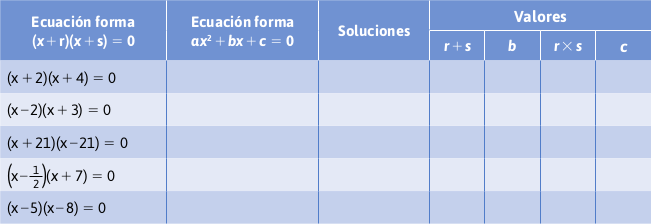
\includegraphics[width=0.9\textwidth]{table2.7.png}
              \captionof{table}{}
              \label{tab:table2.7}
          \end{figure}

    \item Completa la tabla \ref{tab:table2.8}.

          \begin{figure}[H]
              \centering
              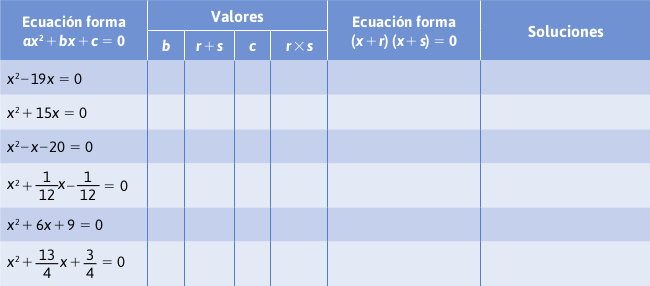
\includegraphics[width=0.9\textwidth]{table2.8.png}
              \captionof{table}{}
              \label{tab:table2.8}
          \end{figure}

    \item Analiza las ecuaciones $2x^2 + 3x - 2 = 0$ y $x^2 + 3 x - 1 = 0$.
          \begin{enumerate}
              \item ¿Observas alguna semejanza entre ambas? ¿Cuál?
              \item ¿Cuáles son las soluciones a la ecuación $x^2 + 3 x - 1 = 0$? Verifica tu respuesta.
              \item Las soluciones que encontraste, ¿son solución de $2x^2 + 3x - 2 = 0$? Explica
              \item ¿Las ecuaciones $2x^2 + 3x - 2 = 0$ y $x^2 + 3 x - 1 = 0$ son equivalentes? ¿Por qué?
          \end{enumerate}
          ¿Cómo dividen una ecuación $ax^2 + bx + c = 0$ entre $a$? ¿Siempre pueden dividir una ecuación
          $ax^2 + bx + c = 0$ entre $a$? ¿Cómo tiene que ser $a$? Consideren que $a$ es un número
          entero, fracción o decimal. Escriban una conclusión en su cuaderno.

    \item Completa la tabla \ref{tab:table2.9}.

          \begin{figure}[H]
              \centering
              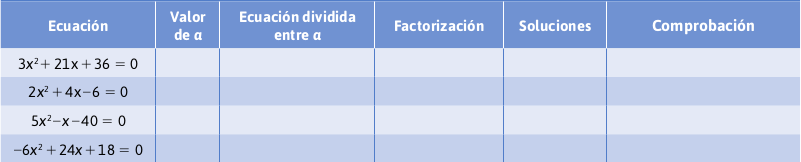
\includegraphics[width=\textwidth]{table2.9.png}
              \captionof{table}{}
              \label{tab:table2.9}
          \end{figure}

          \begin{enumerate}
              \item Expliquen cómo encontrar las raíces de una ecuación del tipo $ax^2 + bx + c = 0$.
              \item Comenten acerca del procedimiento para encontrar las raíces de $ax^2 + bx + c = 0$. Escriban una conclusión en su cuaderno.
          \end{enumerate}

          \begin{boxH}
              Una \textbf{ecuación cuadrática general} del tipo $ax^2 + bx + c = 0$, con $a$, $b$, $c$ números en-
              teros, fraccionarios o decimales y $a \neq 0$, es equivalente a la ecuación $x^2 + \frac{b}{a} x + \frac{c}{a} = 0$,
              la cual se puede factorizar buscando números cuya suma sea igual a $-\frac{b}{a}$ y cuyo
              producto sea igual a $\frac{c}{a}$.
          \end{boxH}

          \subsubsection{Problemas de factorización de ecuaciones cuadráticas}

    \item Escribe la ecuación cuadrática que tenga las raíces indicadas.
          \begin{enumerate}
              \item -1 y 3.
              \item 0 y -17.
              \item -8 y 8.
              \item 11 y 12.
          \end{enumerate}

    \item Resuelve las ecuaciones.
          \begin{enumerate}
              \item $x^2 -  x  - 20 = 0$.
              \item $x^2 + 9x  - 36 = 0$.
              \item $x^2 + 10x + 21 = 0$.
              \item $x^2 + 4x  - 32 = 0$.
          \end{enumerate}

          \begin{minipage}[t]{0.35\textwidth}
              \begin{figure}[H]
                  \centering
                  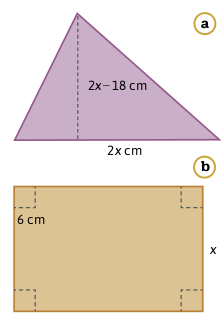
\includegraphics[width=\linewidth]{figuras2.7.png}
                  \captionof{figure}{(a) Triángulo, (b) Pieza rectangular para armar una caja.}
                  \label{fig:figuras2.7}
              \end{figure}
          \end{minipage}\hfill
          \begin{minipage}[t]{0.5\textwidth}
              \item El área de un rectángulo es 28 cm$^2$. Tiene 3 cm más de largo que de ancho. ¿Cuáles son sus dimensiones?
              \item Un terreno rectangular tiene área de 750 m$^2$. Se coloca una cerca alrededor de los 110 m de perímetro. Calcula las dimensiones del terreno.
              \item Un rectángulo tiene el ancho más corto que el largo por 3 cm. El área de la figura es de 51 cm$^2$. ¿Qué medidas tiene?
              \item El triángulo de la figura \ref{fig:figuras2.7}a tiene área igual a 52 cm$^2$, encuentra las medidas de su base y de su altura.
              \item Una pieza rectangular como la de la figura \ref{fig:figuras2.7}b es 4 cm más larga que ancha. Con ella se construye una caja de 840 cm$^3$ cortando un cuadrado
              en cada esquina y doblando los bordes. Escribe las medidas de la altura y el volumen de la caja, así como los lados de la pieza rectangular.

          \end{minipage}

\end{enumerate}


\begin{boxK}
    \begin{center}\textbf{Cierre}\end{center}

    \begin{enumerate}
        \item Retoma la situación de la actividad de inicio y responde, completa o corrige
              tus respuestas. ¿Qué pasaría con el ancho del camino y el área verde si el
              valor de $x$ se redujera a la mitad?
              Reflexiona acerca de los conocimientos o las habilidades que necesitabas al
              inicio y que ahora has adquirido. Escribe en tu cuaderno una conclusión.
        \item Dentro de 15 años, la edad de Elena en ese entonces multiplicada por 6 será
              un tercio del cuadrado de la edad actual. ¿Cuántos años tiene Elena hoy?

              \begin{enumerate}
                  \item Escribe una ecuación que describa el problema.
                  \item ¿Hay más de una solución? Explica por qué y escríbelas, si es el caso.
              \end{enumerate}
    \end{enumerate}
\end{boxK}

\newpage

\subsection{Fórmula general de la ecuación de segundo grado}

\begin{boxK}
    \begin{center}\textbf{Inicio}\end{center}
    \begin{enumerate}
        \item Lee la situación, observa la imagen de la figura \ref{fig:ayb} y responde lo que se pide.
              \begin{figure}[H]
                  \centering
                  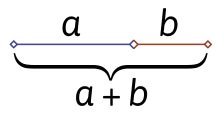
\includegraphics[width=0.4\textwidth]{ayb.png}
                  \captionof{figure}{}
                  \label{fig:ayb}
              \end{figure}
              \begin{boxF}
                  Dos números a y b, distintos de 0, están en proporción áurea si se cumple que:
                  \[\dfrac{a + b}{a}=\dfrac{a}{b}\]
                  de donde, después de hacer algunos cálculos, se obtiene la expresión
                  \[ \left(\dfrac{a}{b}\right)^2-\left(\dfrac{a}{b}\right)-1=0\]
                  en la que $\frac{b}{a}$ es la razón áurea. ¿Cuál es este valor?
              \end{boxF}
              \begin{enumerate}
                  \item Si consideramos que $\frac{b}{a}$ se puede representar por otra variable, por ejemplo $x$, entonces, ¿cómo se escribe la ecuación?
                  \item Los valores $\dfrac{1+\sqrt{5}}{2}$ y $\dfrac{1-\sqrt{5}}{2}$, ¿son soluciones de la ecuación?
                  \item Factoriza la ecuación.
                  \item ¿Cómo piensas que se podría resolver esta ecuación sin factorizar?
                  \item ¿Qué información es relevante para responder y cuál no?
                  \item Describe el procedimiento que realizaste para saber las respuestas.
              \end{enumerate}
    \end{enumerate}
\end{boxK}

\subsubsection{Fórmula general para resolver ecuaciones cuadráticas}
La fórmula general sirve para resolver ecuaciones de segundo grado de todo tipo.

\begin{enumerate}
    \item Considera la ecuación $3x^2 - 7x - 6 = 0$.
          \begin{enumerate}
              \item Encuentra las soluciones de la ecuación. Verifica que lo sean.
              \item Compara la ecuación $3x^2 - 7x - 6 = 0$ con la forma general de una cuadrática $ax ^2 + bx + c = 0$. ¿Cuáles son los valores de $a$, $b$ y $c$?
              \item Sustituye los valores anteriores en las siguientes expresiones. Realiza las operaciones necesarias para resolver y escribe las soluciones obtenidas.

                    $ x_1= \dfrac{-b+\sqrt{b^2-4ac}}{2a} = $ \\[3ex]
                    $ x_2= \dfrac{-b-\sqrt{b^2-4ac}}{2a} = $
              \item Compara tus resultados con los del inciso a). ¿Qué observas?
          \end{enumerate}

    \item Consideren la ecuación $3x^2 + 25x - 28 = 0$.
          \begin{enumerate}
              \item Comparen la ecuación con la forma general de una ecuación cuadrática. Anoten
                    los valores de:

                    $a =$ \rule{15mm}{0.2mm}\\
                    $b =$ \rule{15mm}{0.2mm}\\
                    $c =$ \rule{15mm}{0.2mm}\\

              \item Sustituye los valores de $a$, $b$ y $c$ en las expresiones siguientes. Realiza las operaciones necesarias para resolver y escribe las soluciones obtenidas.

                    $ x_1= \dfrac{-b+\sqrt{b^2-4ac}}{2a} = $ \\[3ex]
                    $ x_2= \dfrac{-b-\sqrt{b^2-4ac}}{2a} = $

              \item  Escriban los valores obtenidos de $x_1$ y $x_2$ con una aproximación de dos decimales.
              \item ¿Cómo pueden verificar que $x_1$ y $x_2$ son soluciones de la ecuación $3x^2 + 25x - 28 = 0$? ¿Qué observan al hacer esta verificación?
          \end{enumerate}

          \begin{boxH}
              Las soluciones $x_1$ y $x_2$ de una ecuación cuadrática de la forma $ax^2 + bx + c = 0$ están dadas por las expresiones
              \[ x_1= \dfrac{-b+\sqrt{b^2-4ac}}{2a} \text{ y }  x_2= \dfrac{-b-\sqrt{b^2-4ac}}{2a}\]
              que se pueden escribir en una sola expresión:
              \[x= \dfrac{-b\pm\sqrt{b^2-4ac}}{2a}\]
              en la que el signo $\pm$ (más menos) indica que para obtener una raíz se suma - b y
              $\sqrt{b^2 - 4ac}$ y para obtener la otra se resta $- b$ y $\sqrt{b^2 - 4ac}$. Esta última expresión se
              conoce como \textbf{fórmula general} para resolver ecuaciones de segundo grado.
          \end{boxH}

          \newpage

    \item Hagan los cálculos en su cuaderno y anoten sus resultados aquí, para obtener las soluciones para cada ecuación e la siguiente tabla.

          \begin{figure}[H]
              \centering
              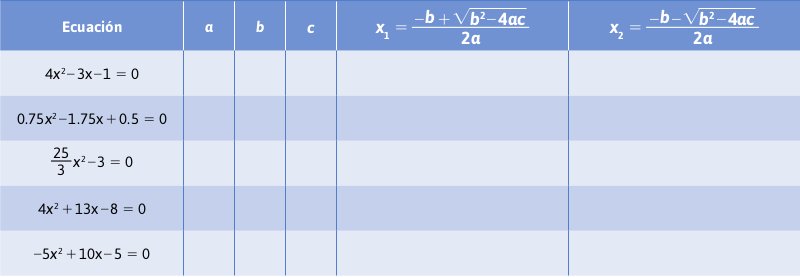
\includegraphics[width=\textwidth]{table2.10.png}
              \captionof{table}{}
              \label{tab:table2.10}
          \end{figure}

    \item Resuelvan las ecuaciones con el método que cada uno prefiera:

          \begin{enumerate}
              \item $3x^2  - 2x - 4 = 0$.
              \item $2x^2 - 5x + 2 = 0$.
              \item $x^2 - x - 6 = 0$.
              \item $x^2 + 2x + 1 = 0$.
              \item $9x^2 - 42x + 40 = 0$.
              \item $0.4^2 - 2x - 3 = 0$.
              \item $\frac{3}{4}x^2 + 6x - 3 = 0$.
              \item $x^2 - 2x - 3 = 0$.
          \end{enumerate}

          En su cuaderno, expliquen en qué casos usaron la fórmula general y por qué. ¿Usaron otros métodos de solución? ¿Cuáles? ¿Por qué?

    \item Se quiere construir una ventana en la que su perímetro y área
          están determinados de antemano (figura 2.8). ¿Cuáles debe ser sus dimensiones?
          \begin{enumerate}
              \item ¿De qué manera expresas algebraicamente el largo del rectángulo? ¿Y su ancho? Explica.
              \item Escribe una ecuación cuadrática que describa el problema.
              \item Escribe las soluciones de la ecuación.
              \item ¿Cuáles son las medidas de la ventana?
          \end{enumerate}

          \newpage

          \subsubsection{Discriminante}
          El discriminante permite determinar si una ecuación cuadrática tiene ninguna, una o
          dos soluciones.

    \item Responde a los siguientes incisos.
          \begin{enumerate}
              \item Consideren la ecuación $x^2 - 6x + 5 = 0$. Realicen lo que se pide. Hagan las operaciones en su cuaderno y anoten los resultados aquí.
                    \begin{itemize}
                        \item Ubiquen los valores de a, b y c correspondientes a la ecuación $x^2 - 6x + 5 = 0$ y obtengan sus soluciones.
                        \item ¿Cuál es el valor de la expresión $b^2 - 4ac$? ¿Se puede calcular $\sqrt{b^2 - 4ac}$? ¿Por qué?
                        \item ¿Observan alguna relación entre el valor de $b^2 - 4ac$ y el número de soluciones de la ecuación $x^2 - 6x + 5 = 0$? ¿Cuál?
                    \end{itemize}

              \item Consideren la ecuación $3x^2 + 24x + 48 = 0$. Hagan las operaciones en su cuaderno y anoten los resultados aquí.
                    \begin{itemize}
                        \item Ubiquen los valores de $a$, $b$ y $c$ correspondientes a la ecuación $3x^2 + 24x + 48 = 0$ y obtengan sus soluciones.
                        \item ¿Cuál es el valor de la expresión $b^2 - 4ac$? ¿Se puede calcular $\sqrt{b^2 - 4ac}$? ¿Por qué?
                        \item ¿Observan alguna relación entre el valor de $b^2 - 4ac$ y el número de soluciones de la ecuación $3x^2 + 24x + 48 = 0$? ¿Cuál?
                    \end{itemize}

              \item Consideren la ecuación $\frac{1}{2}x^2 + 5x + 15 = 0$. Hagan las operaciones en su cuaderno y anoten los resultados aquí.
                    \begin{itemize}
                        \item Ubiquen los valores de $a$, $b$ y $c$ correspondientes a la ecuación $\frac{1}{2}x^2 + 5x + 15 = 0$ y obtengan sus soluciones.
                        \item ¿Cuál es el valor de la expresión $b^2 - 4ac$? ¿Se puede calcular $\sqrt{b^2 - 4ac}$? ¿Por qué?
                        \item ¿Observan alguna relación entre el valor de $b^2 - 4ac$ y el número de soluciones de la ecuación $\frac{1}{2}x^2 + 5x + 15 = 0$? ¿Cuál?
                    \end{itemize}
          \end{enumerate}

    \item Completa la tabla \ref{tab:table2.11}.

          \begin{figure}[H]
              \centering
              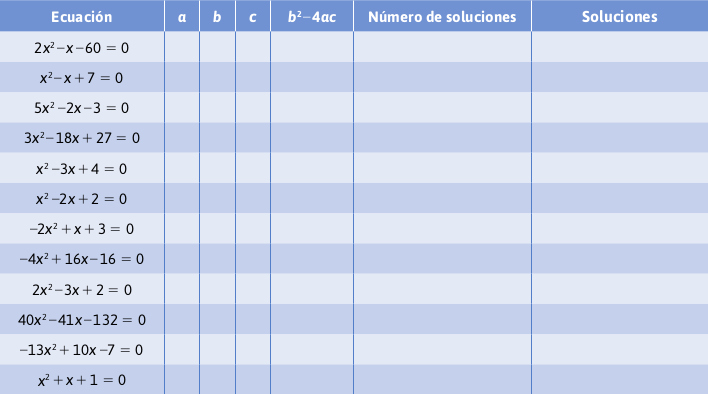
\includegraphics[width=\textwidth]{table2.11.png}
              \captionof{table}{}
              \label{tab:table2.11}
          \end{figure}

          \begin{enumerate}
              \item Si $b^2 - 4ac = 0$, ¿cuántas soluciones tiene la ecuación cuadrática? ¿Por qué?
              \item Sí $b^2 - 4ac > 0$, ¿cuántas soluciones tiene la ecuación cuadrática? ¿Por qué?
              \item Si $b^2 - 4ac < 0$, ¿cuántas soluciones tiene la ecuación cuadrática? ¿Por qué?
              \item ¿Cuál es la importancia de calcular $b^2 - 4ac$? Escriban una conclusión en su cuaderno.
          \end{enumerate}

          \begin{boxH}
              La ecuación cuadrática $ax^2 + bx + c = 0$ tiene:
              \begin{itemize}
                  \item Dos soluciones si $b^2 - 4ac > 0$ y las raíces son

                        \[x_1 = \frac{-b + \sqrt{b^2 - 4ac}}{2a} \text{ y } x_2 = \frac{-b - \sqrt{b^2 - 4ac}}{2a}\]

                  \item Una solución si $b^2 - 4ac = 0$ y la raíz es

                        \[x = \frac{-b}{2a}\].

                  \item Ninguna solución real si $b^2 - 4ac < 0$.
              \end{itemize}

          \end{boxH}

          \begin{boxH}
              A la expresión \textbf{$b^2 - 4ac$} se le conoce como el \textbf{discriminante} de la ecuación
              cuadrática.
          \end{boxH}
\end{enumerate}

\newpage

\subsubsection{Problemas con ecuaciones de segundo grado}

\begin{enumerate}
    \item Contesta.
          \begin{enumerate}
              \item ¿Cuántas raíces tiene la ecuación $9x^2 - 2x + 4 = 0$?
              \item Escribe una ecuación que tenga soluciones $x_1 = 0.3$ y $x_2 = 0.7$.
              \item Anota una ecuación que tenga una sola solución $x = -3$.
          \end{enumerate}

    \item Si al producto de un número natural por su consecutivo le restamos 31, obtenemos
          el quíntuple de la suma de ambos. ¿De qué números se trata?

    \item Un proyectil es lanzado verticalmente y la expresión $h(t) = 512t - 16t^2$ describe la
          altura $h$ de su posición después de $t$ segundos.
          \begin{enumerate}
              \item ¿Qué altura alcanza después de 6 segundos?
              \item ¿El proyectil alcanza la altura de 3,520 m? Si es así, ¿en qué tiempo la alcanza?
              \item ¿En qué momento alcanza la altura de 5,500 m?
              \item ¿En cuánto tiempo regresará a la tierra? Explica.

          \end{enumerate}

    \item Un terreno rectangular tiene dimensiones de 8 m por 24 m. Si el ancho y el largo
          aumentan en una misma cantidad fija, el área aumenta 144 m$^2$. ¿Cuántos metros
          aumentan el largo y el ancho del terreno?
          \begin{enumerate}
              \item ¿Cuántos metros aumentaron las dimensiones?
              \item ¿Cuáles son las nuevas medidas del largo y el ancho?
          \end{enumerate}

    \item Si $P$ pesos se invierten a dos años con un interés anual $x$; a ese interés, la inversión
          crecerá a otra cantidad $A$, también en pesos, mediante la fórmula $A = P(1 + x)^2$.
          ¿A qué tasa de interés $x$, una cantidad inicial de \$1,000.00 crecerá a \$1,200.00 en los dos años?

    \item Dos automóviles viajan a velocidades uniformes sobre la misma ruta cubriendo una distancia de 180 km. Uno va 5 km más despacio que otro y tarda 30 min más en hacer el recorrido. ¿A qué velocidad va cada automóvil?

    \item En un concurso de matemáticas, se planteó un problema sobre una ecuación de segundo grado. Un estudiante lo resuelve pero se equivoca en el término independiente (c) y obtiene como soluciones: 9 y 3. Otro estudiante se equivoca en el coeficiente del término de primer grado (b) y obtiene como soluciones: -7 y -5. ¿Cuál fue la ecuación planteada del problema?


\end{enumerate}

\begin{boxK}
    \begin{center}\textbf{Cierre}\end{center}

    \begin{enumerate}
        \item Retoma la situación de la actividad de inicio y responde, completa o corrige tus respuestas. ¿Qué pasaría si en la razón, se cambia $a - b$ en lugar de $a + b$?
              ¿Es más fácil resolver la ecuación? ¿Por qué?
              Reflexiona acerca de los conocimientos o las habilidades que necesitabas al inicio y que ahora has adquirido. Escribe en tu cuaderno una conclusión.
        \item El sistema romano de proporciones arquitectónicas se basa
              en el llamado número de plata. Un rectángulo cuya relación entre los lados sea igual al número de plata se denomina
              rectángulo plateado. Resuelve la ecuación $x^2 - 2x - 1 = 0$ para conocer su valor. ¿Cuántas soluciones tiene? ¿Qué solución es la que tiene sentido? Explica.
    \end{enumerate}

    \begin{figure}[H]
        \centering
        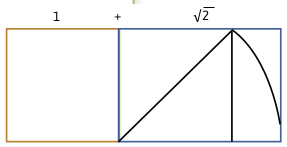
\includegraphics[width=0.6\textwidth]{plata.png}
        \captionof{figure}{Rect\'angulo de plata.}
        \label{fig:plata}
    \end{figure}

\end{boxK}

\begin{boxF}
    Los matemáticos de la antigüedad buscaron cómo definir la belleza y
    establecieron que una figura que tenga proporción áurea nos resultará
    preciosa y hermos a. Denominaron a esta proporción el número de oro
    $\Phi$ (fi). Para calcularlo se basaron en una definición: una forma es bella
    cuando la proporción entre el total y su parte mayor (razón extrema) es
    igual a la proporción entre su parte mayor y su parte menor (razón media).
    Éste es el concepto de belleza que tomó \textbf{Leonardo da Vinci (1452-
        1519)} en su famosa obra \emph{El hombre de Vitruvio}. Con base en la figura,
    calcula el valor del número de oro.

    \[ \frac{\Phi+1}{\Phi} = \frac{\Phi}{1} \]

    \begin{figure}[H]
        \centering
        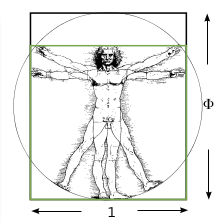
\includegraphics[width=0.4\textwidth]{hombre.png}
        \captionof{figure}{Bosquejo de \emph{El hombre de Vitruvio} por Leonardo da Vinci.}
        \label{fig:hombre}
    \end{figure}

\end{boxF}

\newpage